% ============================================================================
% main.tex -- "Where to better live in Milan: neighbourhood differentiation
% and the M4 creation case"
%
% Built on the official PNAS Overleaf template (2025), class pnas-new with
% \templatetype{pnasresearcharticle}. The class and style files (pnas-new.cls,
% pnasresearcharticle.sty, pnas-new.bst, widetext.sty, PNAS logos) are NOT
% redistributed here: open the official template on Overleaf
%   https://www.overleaf.com/latex/templates/template-for-preparing-your-research-report-submission-to-pnas-using-overleaf-2025/whbdryzwztnd
% ("Open as Template"), then upload main.tex, references.bib and the
% figures/ folder into that project (replace the template's main file).
%
% Structure: IMRaD as requested by the instructor (Methods BEFORE Results).
% The template's \matmethods{} block, which PNAS typesets at the end, is not
% used; Methods is an ordinary section placed after the Introduction.
%
% Abstract and Literature Review: verbatim from the group draft
% ("Housing affordability Milan (1).docx"). Only technical changes needed by
% LaTeX were made (% escaped as \%). The Literature Review keeps its
% author-year citations as plain text; the corresponding entries are added to
% the reference list with \nocite (see the end of the file).
% ============================================================================

\documentclass[9pt,twocolumn,twoside]{pnas-new}
% Use the lineno option to display guide line numbers if required.

\articletype{Social Sciences: Economic Sciences}% CHECK: PNAS classification

\templatetype{pnasresearcharticle} % two-column research article

\usepackage{booktabs}  % already loaded by the class in recent versions; harmless if repeated

\begin{document}

\title{Where to better live in Milan: neighbourhood differentiation and the M4 creation case}

% TO COMPLETE: affiliations, order of authors, corresponding author.
\author[a]{Salvatore Calaciura}
\author[a]{Mattia Colombo}
\author[a]{Federica Leaci}
\author[a]{Sofia Pangher}
\author[a]{Yigit Yildiz}

\affil[a]{[Affiliation to be completed]}

% Surname of the lead author for the running footer (CHECK)
\leadauthor{Calaciura}

% The template asks for a 50--120-word significance statement. A draft is
% provided separately (significance_statement_DRAFT.txt) for the group's
% approval; it is left empty here so that the Abstract is not altered.
\significancestatement{}

\authorcontributions{[To be completed by the group.]}
\authordeclaration{[To be completed by the group.]}
\correspondingauthor{[To be completed: corresponding author and e-mail.]}

\keywords{housing affordability $|$ Milan $|$ OMI rent quotations $|$ metro line $|$ difference-in-differences}

% ---------------------------------------------------------------------------
% ABSTRACT -- verbatim, do not edit
% ---------------------------------------------------------------------------
\begin{abstract}
Rising rents have fuelled concerns about access to housing in Milan, resulting in widespread protests across the city. This study examines how rental affordability has evolved across the city’s neighbourhoods and whether the opening of the M4 metro line affected affordability in nearby areas. We construct a neighbourhood-level index comparing estimated annual rents for a standard dwelling with a common citywide reference income, identifying where and when rental costs exceeded a 40\% benchmark. We then apply a difference-in-differences approach that accommodates staggered station openings, comparing changes near M4 stations with those in comparable neighbourhoods elsewhere in Milan. By combining affordability trends with an evaluation of a specific infrastructure investment, the study extends existing evidence on the geography and evolution of housing access in Milan. The analysis will inform discussion of how transport improvements can be coordinated with housing policies, while distinguishing changes in rental affordability from direct evidence of residential displacement.
\end{abstract}

\dates{This manuscript was compiled on \today}
\doi{\url{www.pnas.org/cgi/doi/10.1073/pnas.XXXXXXXXXX}}

\maketitle
\thispagestyle{firststyle}
\ifthenelse{\boolean{shortarticle}}{\ifthenelse{\boolean{singlecolumn}}{\abscontentformatted}{\abscontent}}{}

\Firstpage

% ============================================================================
% INTRODUCTION
% ============================================================================
\section*{Introduction}

Recent protests over rising rents have placed housing affordability at the centre of public debate in Milan and across Europe. These concerns raise a central empirical question: to what extent has it become more difficult for a person on a typical local income to rent a home in the city, and where? This paper addresses the question in two steps.

First, we measure how rental affordability has evolved across Milan's neighbourhoods (Nuclei di Identit\`a Locale, NIL). We construct an index that relates the quoted annual rent of a standard 60~m$^2$ dwelling in each neighbourhood to a single citywide reference income, the simulated median net income of Milanese taxpayers, and we identify the neighbourhoods and years in which this rent exceeds 40\% of that income, the threshold used by the OECD to define housing cost overburden \cite{oecd2024}. Because the denominator is common to all neighbourhoods, the index describes where a person with the benchmark income could afford to rent; it is not the rent burden of current residents.

Second, we ask whether public transport investment contributed to these rent dynamics. Better access to transit lowers commuting costs and, according to the capitalisation of accessibility, raises the price of housing near new stations \cite{alonso1964,gibbons2005}; empirical studies of new rail lines generally find positive but modest and very local effects \cite{billings2011}, and in Italy Daniele and Romito \cite{daniele2022} use OMI zone quotations, the data source we also rely on, to study the opening of Metro C in Rome. Milan's M4 line, which opened in three stages between November 2022 and October 2024, offers a staggered natural experiment in the middle of our study period. We estimate its effect on the rent quotations of the areas it served for the first time with a heterogeneity-robust difference-in-differences design \cite{callaway2021} and randomisation inference suited to a small number of treated areas.

The two parts answer three research questions: (\textit{i}) how has rental affordability evolved across Milan's neighbourhoods between 2015 and 2024? (\textit{ii}) in which neighbourhoods, and from when, did the rent of a standard dwelling exceed 40\% of the median taxpayer's net income? (\textit{iii}) did the opening of the M4 raise rents in newly served areas relative to comparable areas elsewhere in the city?

We find that the share of residents living in neighbourhoods out of reach for a single median earner was broadly stable between 2015 and 2022, at 25--30\%, and then rose to 43\% in 2024, because quoted rents grew much faster than incomes. Unaffordability is concentrated in the city centre and its first ring, but the index rose in the periphery as well. For the M4, we find no robust evidence of an increase in rent quotations in the five newly served OMI zones over the first three to seven semesters after opening: relative increases larger than about 2\% are inconsistent with the data, while the design cannot distinguish a zero effect from a moderate decrease. The 2022--2024 deterioration in affordability therefore does not appear to be concentrated around the new stations.

The paper proceeds as follows. The Literature Review below situates the study. Methods describes the data, the affordability index and the design of the M4 analysis; Results presents the affordability evidence and the M4 estimates; Discussion interprets both, sets out their limitations and concludes. Alternative specifications and sensitivity analyses are reported in the Appendix.

% ---------------------------------------------------------------------------
% LITERATURE REVIEW -- verbatim, do not edit (headings included)
% ---------------------------------------------------------------------------
\subsection*{Literature Review}

\subsubsection*{2.1 Conceptualising housing affordability}

Housing affordability concerns the relationship between housing costs and the economic resources available to households, thus we decided to employ rent-to-income ratios, which constitute a transparent measure that facilitates comparison across space and time, albeit their limited interpretive depth. Banca d'Italia (2026) provides the closest methodological precedent to the present study, comparing OMI rental midpoints for a standard dwelling with average net taxpayer income. Our index adapts this approach in order to examine neighbourhood-level differences over time using a common citywide reference income.

Additionally, Hulchanski (1995) distinguishes the descriptive use of expenditure ratios from the assessment of housing need, while the Scottish Government (2019) draws attention to variation in affordability thresholds and household circumstances. The OECD (2024) defines housing cost overburden as expenditure exceeding 40\% of disposable household income on housing. Although this offers a useful reference benchmark, its application necessitates a clear distinction between household disposable income and gross taxpayer income.

\subsubsection*{2.2 Affordability pressures in Milan and the role of public investment}

A growing body of research documents intensifying affordability pressures in Milan. Bricocoli and Peverini (2024) demonstrate that housing costs have increased faster than incomes and wages. Bricocoli, Peverini and Caresana (2025) extend this analysis to the surrounding urban region, arguing that commuting costs should be incorporated into assessments of ostensibly cheaper peripheral housing.

Public investment may shape these patterns by enhancing neighbourhood attractiveness. Zheng and Kahn (2013) associate infrastructure improvements in Beijing with higher property values, increased housing development, and socioeconomic upgrading. Nevertheless, market responses may precede the operation of the infrastructure itself: McMillen and McDonald (2004) document anticipation effects associated with Chicago's Midway Line, a limitation acknowledge in our M4 analysis. Melser (2020) contends that rents may reflect currently available infrastructure services more directly than sale prices, while acknowledging structural differences between rental and owner-occupied markets. Building on this literature, we combine a spatial and temporal assessment of rental affordability with a case study of the M4 line. The empirical strategy draws on the framework of Callaway and Sant'Anna (2021), which accommodates staggered treatment timing and heterogeneous treatment effects, conditional on the validity of its identifying assumptions.

\subsubsection*{2.4 Heterogeneity and the limits of inference}

The relationship between infrastructure investment and exclusion is, however, contingent upon local conditions and accompanying policy measures. Padeiro, Louro and Marques da Costa (2019) identify methodological weaknesses in the literature on transit-induced gentrification. In the Milanese context, Bricocoli and Cucca (2016) question whether social mixing necessarily enhances housing inclusion, while Bortolotti and Grassi (2025) highlight inequalities in participation within regeneration processes.
% --- end of verbatim Literature Review ---

% ============================================================================
% METHODS
% ============================================================================
\section*{Methods}

The paper uses two geographies, chosen to match the level at which each outcome is recorded. The affordability index is computed for neighbourhoods (NIL), the municipal units at which population is recorded, so that rents can be summarised by the number of residents exposed to them. The M4 analysis is conducted on OMI zones, the units at which rent quotations are originally published: averaging zone quotations into neighbourhoods would add no information on rents, would mechanically mix served and unserved zones, and would overstate the number of independent observations available for inference.

\subsection*{Data Sources}

\paragraph{Housing quotations.} Rents come from the semi-annual quotations of the Osservatorio del Mercato Immobiliare (OMI) of the Agenzia delle Entrate, available through Milan's open-data portal (dataset DS1996) \cite{comune_opendata} and supplemented with the Agency's release for the first half of 2026 \cite{agenziaentrate_omi}. For each OMI zone and semester, OMI publishes a minimum and a maximum value for ordinary residential dwellings (\textit{abitazioni civili}, OMI category 20) in normal condition. We use the midpoint of each interval: rents in euros per square metre of gross floor area per month, sale prices in euros per square metre. These are area-level reference quotations based on appraisals, not rents paid by individual households or transaction prices.

\paragraph{Zoning.} OMI zone boundaries changed in 2014: until 2013 Milan was divided into 55 zones with different boundaries, and the first semester of 2014 is a transition period in which part of the city still carries the old codes. We therefore use quotations from 2014S2 onwards. In the second half of 2024 OMI split two peripheral zones (D15 into D37 and D38, D30 into D39 and D40); we map the new zones back to the 2014 boundaries using area weights, so that each original zone's quotation is the area-weighted average of its successors. Neither zone is part of the M4 estimation sample.

\paragraph{Income, population and stations.} Income comes from the municipal distribution of taxpayers across total-income classes (DS531), and aggregate tax liabilities from DS312. Resident population by neighbourhood comes from the municipal registry (DS205), and neighbourhood composition by age, citizenship and household type from DS27 and DS1440. Metro station coordinates and line membership come from DS535 \cite{comune_opendata}.

\subsection*{Neighbourhood Rents}

We map OMI quotations to current NIL boundaries using intersection-area weights, approximated by a regular grid of points with a spacing of about 28 metres. Each semester is linked to the zoning map in force in that semester. For NIL $i$ in semester $s$, rent and spatial coverage are
\begin{equation}
R_{is}=\frac{\sum_{z\in Q_s} n_{izs}\,R_{zs}}{\sum_{z\in Q_s} n_{izs}},\qquad
C_{is}=\frac{\sum_{z\in Q_s} n_{izs}}{N_i},
\label{eq:nilrent}
\end{equation}
where $n_{izs}$ counts the grid points of NIL $i$ falling in OMI zone $z$ under the zoning in force in semester $s$, $Q_s$ is the set of zones with a valid quotation in that semester, $R_{zs}$ is the quotation midpoint and $N_i$ counts all grid points in the NIL. Only quoted areas enter the average, and a NIL-semester is retained when $C_{is}\ge0.80$. The weights are surface weights, so non-residential land counts towards coverage and the neighbourhood rent is not weighted by dwellings or tenants. The area later quoted as zone C14 (Porta Nuova), carved out of zone C12, receives the C12 quotation until 2018S1, before separate C14 quotations become available in 2018S2.

Annual rents average the two semesters of each year. The index starts in 2015, the first full year under the current zoning, because 2014 has only one valid semester; it ends in 2024, the last tax year for which income data are available. We retain the NILs with at least 500 residents in 2019 and a rent observed in every year from 2015 to 2024. The balanced sample comprises 75 NILs and 750 NIL-year observations.

\subsection*{Median Income Benchmark}

The denominator is a single citywide income, not a neighbourhood income. We use the distribution of Milanese taxpayers across total-income classes (DS531, tax years 2015--2024); income is aligned with rents by tax year. Class frequencies identify the class containing the median taxpayer, and interpolation assumes a uniform distribution within that class. Because net income increases monotonically with gross income, we transform the endpoints of the median class into net values and interpolate between them:
\begin{equation}
\tilde Y_t=f_t(L_t)+\frac{N_t/2-B_t}{n_t}\left[f_t(U_t)-f_t(L_t)\right],
\label{eq:netincome}
\end{equation}
where $L_t$ and $U_t$ are the class endpoints, $N_t$ is the number of taxpayers, $B_t$ the number of taxpayers below the median class, $n_t$ its frequency and $f_t$ the year-specific gross-to-net transformation. Net income equals total income minus national personal income tax and the regional and municipal surcharges, plus the in-work tax bonus. Because DS531 does not record whether a taxpayer is an employee, a pensioner or self-employed, the baseline applies the tax credits for employees; it excludes household-specific deductions (dependants, medical expenses, mortgages) and transfers not recorded in tax returns. $\tilde Y_t$ is therefore a simulated individual income at the median taxpayer rank, not observed median household disposable income. Applied to all taxpayers, the employee schedule implies an average tax rate of about 31\% of total income in 2015--2024, against about 27\% in the taxes actually paid (DS312): the baseline overstates taxes because deductions that are not modelled are actually claimed. The Appendix shows how the results change under other tax assumptions, including a scenario calibrated to the taxes actually paid.

\subsection*{Affordability Index}

For a standard dwelling of 60~m$^2$, the index compares annual quoted rent with median net income:
\begin{equation}
A_{it}=\frac{12\times60\times R_{it}}{\tilde Y_t}.
\label{eq:index}
\end{equation}
Higher values indicate lower affordability. A NIL is classified as out of reach when $A_{it}>0.40$, drawing on the OECD housing cost overburden convention, which counts households spending more than 40\% of their disposable income on housing \cite{oecd2024}. For each year we report the share of the 75 NILs above the threshold and the share of residents living in them, using annual resident counts (DS205) as weights and the population of the 75 NILs as denominator. This summary is not an official overburden rate: it uses a hypothetical dwelling, quoted rents and a simulated individual income instead of observed household costs and disposable income. Rents and income are both in current euros; deflating both by the same price index would leave their ratio unchanged. Two household scenarios rescale the index: one median earner in a 40~m$^2$ dwelling ($A^{40}_{it}$) and two median earners in a 60~m$^2$ dwelling ($A^{60d}_{it}$).

\subsection*{The M4 Line: Treatment Definition and Timing}

\paragraph{Panel.} The M4 analysis uses a panel of OMI zones from 2014S2 to 2026S1. We keep the zones with a rent quotation in every semester, a balanced panel of 37 zones over 24 semesters (888 observations). The outcome is the log midpoint rent. Because the affordability index divides every rent by the same citywide income, a difference-in-differences contrast in log rent equals the contrast in log rent-to-income: the M4 analysis measures the line's effect on affordability as defined above.

\paragraph{Exposure.} We overlay a regular grid of points on the city. A point is \textit{newly served} if it lies within 500~m of an M4 station and more than 500~m from any station of the other metro lines (M1, M2, M3, M5). A zone's exposure to an opening section is the share of its grid points newly served by that section's stations. A zone is treated if its exposure reaches 20\%, and \textit{never exposed} if none of its points lies within 500~m of any M4 station; partially exposed zones and zones near the M4 already served by other lines are excluded. The 500~m radius corresponds to the walking catchment of an urban station and is close to the median distance between consecutive M4 stations (469~m).

\paragraph{Timing.} The first treated period of a zone is the first semester during which its section was open for all or almost all of the semester (Table~\ref{tab:m4timing}). Sections 1 and 3 opened late in the year (26 November 2022 and 12 October 2024), so their first treated semesters are 2023S1 and 2025S1. Section 2 newly serves no zone, because its stations (Tricolore and San Babila) are within 500~m of the M1 and M3 lines. Five OMI zones are therefore treated: D12 from 2023S1, with seven post-opening semesters, and B13, B20, B21 and D24 from 2025S1, with three.

\begin{table*}[tbhp]
\centering
\caption{M4 opening dates and treated OMI zones (500~m catchment, 20\% exposure threshold)}
\label{tab:m4timing}
\resizebox{\textwidth}{!}{%
\begin{tabular}{llcccl}
\toprule
Section & Opening date & Opening semester & First treated & Post-opening semesters & Treated zones \\
 & & (share of days open) & semester & to 2026S1 & \\
\midrule
1 Linate--Dateo & 26 Nov 2022 & 2022S2 (20\%) & 2023S1 & 7 & 1 (D12) \\
2 Dateo--San Babila & 4 Jul 2023 & 2023S2 (98\%) & 2023S2 & 6 & 0 \\
3 San Babila--San Cristoforo & 12 Oct 2024 & 2024S2 (44\%) & 2025S1 & 3 & 4 (B13, B20, B21, D24) \\
\bottomrule
\end{tabular}}
\addtabletext{Source: authors' elaboration on OMI and Comune di Milano open data (DS535).}
\end{table*}

\paragraph{Control group.} For each treated zone we select the three never-exposed zones most similar before the metro, by Euclidean distance on standardised covariates: the 2014--2016 levels of log rents and log sale prices, the 2014--2019 growth of log rents, and the 2014 shares of foreign residents, of residents aged 65 and over and of single-person households, mapped from neighbourhoods to zones by area overlap. This yields six matched controls (B15, C19, D18, D20, D28, D36), to which the zones of later sections are added as not-yet-treated controls until they open. The main sample thus contains 11 zones (264 zone-semesters).

\subsection*{Estimand and Identification}

The target parameter is the average effect of gaining new M4 access on the log OMI midpoint rent of the five treated zones, over the semesters observed after their opening, relative to the counterfactual path given by the controls. Identification requires (\textit{i}) parallel trends: absent the line, treated zones and their controls would have followed the same rent path from the reference semester onwards; (\textit{ii}) no anticipation between the reference semester and opening; and (\textit{iii}) no spillovers of the line onto control zones. The estimate is a relative effect, which differences out any effect of the line common to the whole city; it concerns OMI quotations rather than contract rents; and it does not extend beyond the three to seven semesters observed after opening.

\subsection*{Estimator and Event Study}

Because the sections opened at different dates, a two-way fixed-effects regression would use already-treated zones as controls for later-treated ones, which can bias the estimate when effects vary over time \cite{goodmanbacon2021,dechaisemartin2020}. We use instead the estimator of Callaway and Sant'Anna \cite{callaway2021}. Let $g$ be the first treated period of an opening group and $b=g-1$ a common reference period. For log rent $Y$,
\begin{equation}
\mathrm{ATT}(g,t)=\left[\bar Y_{g,t}-\bar Y_{g,b}\right]-\left[\bar Y_{C(g,t),t}-\bar Y_{C(g,t),b}\right],
\label{eq:attgt}
\end{equation}
where the control set $C(g,t)$ contains the sample zones that are never exposed or that open after $\max(t,b)$, and means are unweighted across zones. The headline estimate averages the post-opening effects, weighting each group by its number of treated zones $n_g$:
\begin{equation}
\mathrm{ATT}=\frac{\sum_g\sum_{t\ge g} n_g\,\mathrm{ATT}(g,t)}{\sum_g\sum_{t\ge g} n_g},
\label{eq:attagg}
\end{equation}
so that section 1 (one zone $\times$ 7 semesters) receives weight 7/19 and section 3 (four zones $\times$ 3 semesters) weight 12/19. Aggregating by time relative to opening, $e=t-g$, gives the event study
\begin{equation}
\mathrm{ES}(e)=\frac{\sum_g n_g\,\mathrm{ATT}(g,g+e)}{\sum_g n_g},
\label{eq:es}
\end{equation}
where the sums run over the groups observed at $e$ and $\mathrm{ES}(-1)=0$ by construction. Pre-opening coefficients assess differential trends; their average over $e=-8,\dots,-2$ is reported as a placebo. Coefficients are reported in log points; percentages are $100\times(\exp(\cdot)-1)$.

\subsection*{Inference and Statistical Power}

With five treated zones, cluster-robust standard errors are unreliable \cite{conley2011,mackinnon2018}, so inference is based on randomisation. We test the sharp null that the M4 had no effect on any zone in any semester. In the main sample of 11 zones we randomly reassign the opening-group labels (one zone opening in 2023S1, four in 2025S1, six controls), keeping the number of zones per group fixed, and recompute the full estimator for each of 999 draws, out of 2,310 distinct assignments. The two-sided $p$-value is
\begin{equation}
p=\frac{1+\#\{|\mathrm{ATT}_p|\ge|\mathrm{ATT}|\}}{1+B},
\label{eq:perm}
\end{equation}
with $B=999$; the same procedure gives the $p$-value of the placebo. The test has exact finite-sample level only if, under the null, the observed assignment of opening dates is one equally likely draw among the relabellings. Because the dates were set by the route of the line and the treated zones are central, this exchangeability is a maintained assumption; the test also conditions on the matched sample, which is not re-drawn within permutations.

For the main estimate we obtain a 95\% confidence interval by inverting the permutation test under a constant additive effect \cite{imbens2015}: a value $\delta$ belongs to the interval if the test of no effect applied to $Y-\delta D$, where $D=1$ for treated zones after their own opening, does not reject at the 5\% level. For event-study coefficients and secondary checks we use the faster approximation $\widehat{\mathrm{ATT}}\pm c$, where $c$ is the 95th percentile of the permuted $|$estimates$|$, together with a simultaneous sup-$t$ band \cite{montielolea2019} built from the same permutation distribution over $e=-12,\dots,6$ (critical value $\hat c=2.40$), which covers all coefficients jointly. Under the same constant-effect approximation, the minimum detectable effect with 80\% power is the smallest $\delta$ such that $P(|\delta+e_p|\ge c)\ge0.8$ over the permuted estimates $e_p$. For the main specification $c=0.062$ log points and the minimum detectable effect is 9.4\% (Monte Carlo error about 0.3 percentage points): an effect of about $\pm9\%$ would be detected eight times out of ten, but smaller effects cannot be ruled out.

\subsection*{Robustness and Alternative Estimators}

We assess the main estimate along four dimensions, reported in full in the Appendix: (\textit{i}) the control group, using all 20 never-exposed zones or only not-yet-treated zones; (\textit{ii}) the treatment definition, with catchments of 800 and 1,000~m and exposure thresholds of 10\% and 30\%; (\textit{iii}) influential zones and the classification of opening periods, dropping one treated zone at a time, using $g-2$ as reference so that the partly served semester enters neither the base nor the effects, and dating treatment from the opening semester itself; and (\textit{iv}) the estimator. For the last, we use synthetic difference-in-differences \cite{arkhangelsky2021}, which chooses weights for control zones and pre-opening semesters so that the weighted controls track the treated zones before opening, estimated on the balanced sample of the five treated and 20 never-exposed zones with placebo standard errors (500 replications), and we compare it with Callaway--Sant'Anna and a plain difference-in-differences on the same sample and horizon. A two-way fixed-effects regression with zone and semester fixed effects and standard errors clustered by zone is reported for comparison only.

% ============================================================================
% RESULTS
% ============================================================================
\section*{Results}

\subsection*{How Many Neighbourhoods Are Out of Reach?}

In 2015, 16 of the 75 NILs (21.3\%) were out of reach for a single median earner, and 24.7\% of residents lived in them. The share of NILs stayed between 21.3\% and 26.7\% until 2022, then rose sharply: in 2024, 27 NILs (36.0\%) exceeded the threshold, home to 43.2\% of residents (Fig.~\ref{fig:share}). The share of residents is always higher than the share of NILs because the unaffordable neighbourhoods, around the centre, are more populous on average.

The deterioration reflects rents growing faster than incomes. Between 2015 and 2024 the median NIL rent rose by 45.4\%, from EUR~7.77 to EUR~11.30 per m$^2$ per month, while the median net income rose by 24.1\%, from EUR~17,370 to EUR~21,559. The gap widened after 2022: between 2022 and 2024 rents increased by 30.6\% and income by 9.2\%.

\begin{figure}[tbhp]
\centering
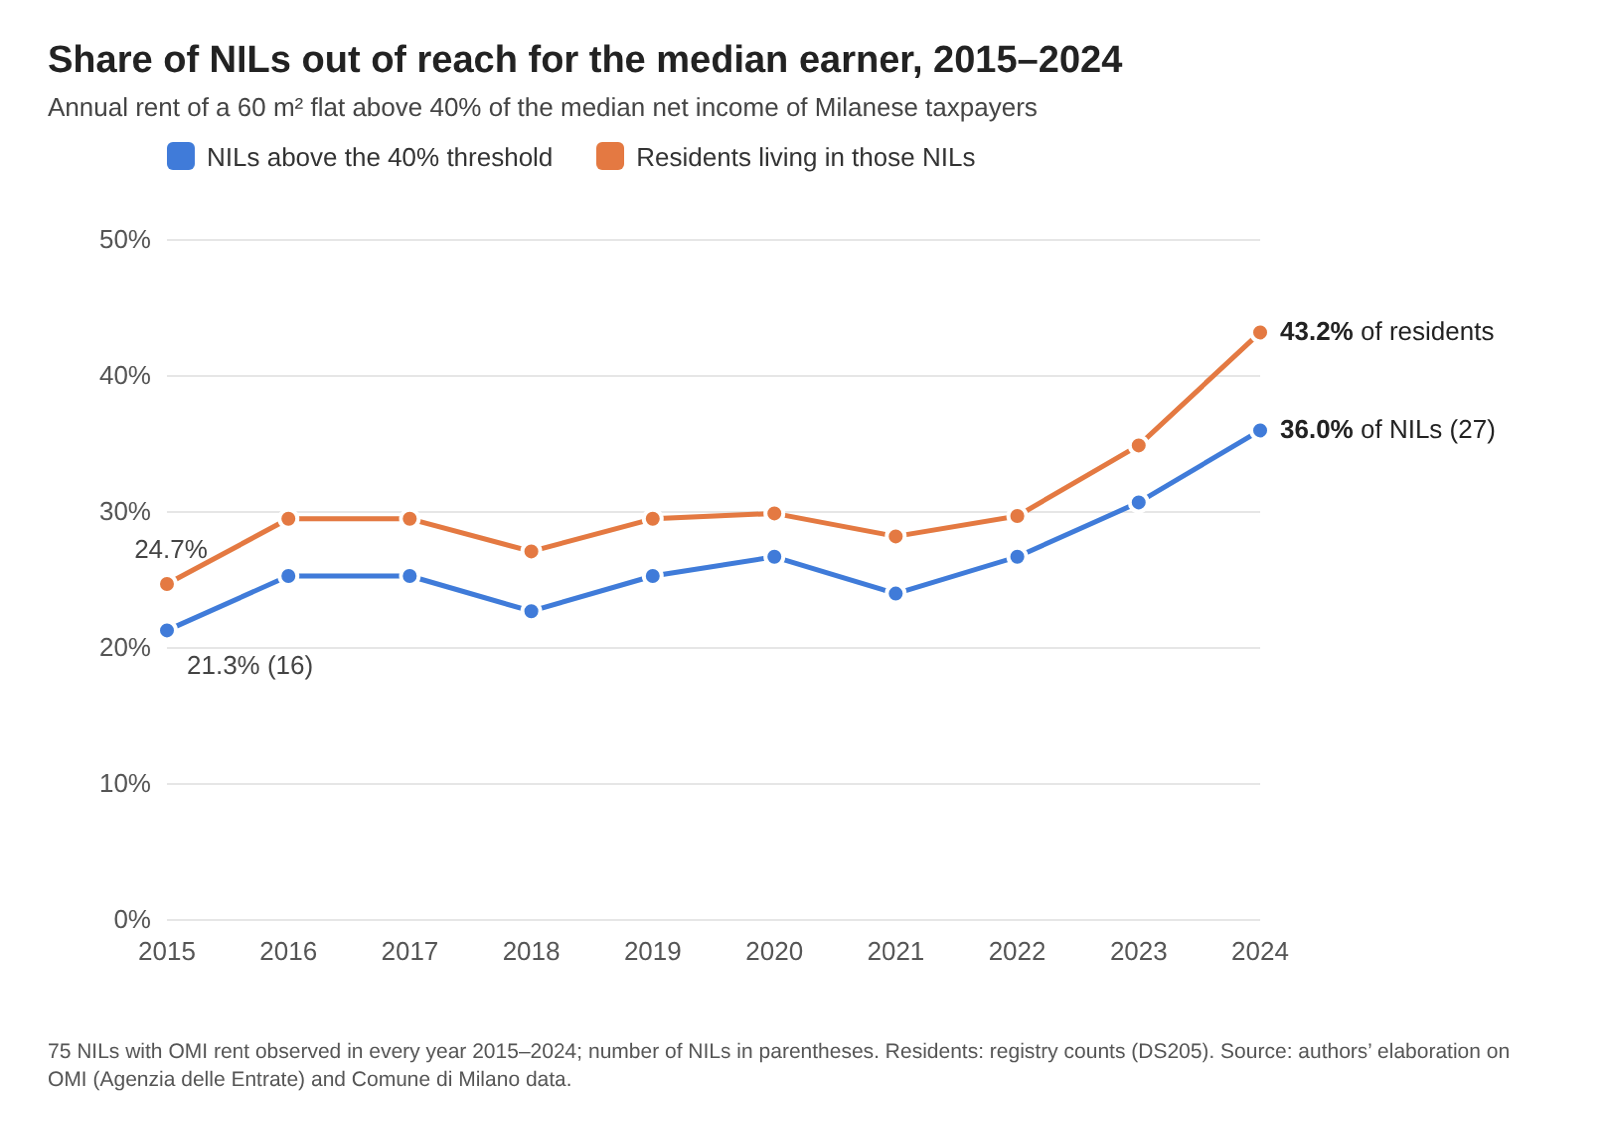
\includegraphics[width=\linewidth]{figures/fig1_share_out_of_reach.png}
\caption{Share of NILs out of reach for the median earner, 2015--2024: NILs where the annual OMI rent of a 60~m$^2$ dwelling exceeds 40\% of the median net income of Milanese taxpayers (blue), and share of residents living in them (orange). Balanced sample of 75 NILs; residents from DS205. Source: authors' elaboration on OMI and Comune di Milano data.}
\label{fig:share}
\end{figure}

\subsection*{Where Are the Most and Least Affordable Neighbourhoods?}

In 2024 the index ranges from 25.7\% to 83.9\%, with a median of 37.7\%. The lower quartile ($A\le36.3\%$) and the upper quartile ($A\ge46.5\%$) each contain 19 NILs (Table~\ref{tab:quartiles}). All lower-quartile NILs are below the threshold and all upper-quartile NILs above it. The most affordable quartile is entirely peripheral: the south (Gratosoglio), the north-west (Quarto Oggiaro, Bovisasca, Comasina, Affori, Bruzzano), the west (Muggiano, Quinto Romano, Baggio, Figino, Trenno, Gallaratese) and the north-east (Adriano, Padova, Gorla); its average rent is EUR~9.96 per m$^2$ and it hosts about 299,000 residents. The least affordable quartile is the city centre and its first ring, from Duomo, Brera and Guastalla to Porta Venezia, Isola, the Navigli and Sarpi, with an average rent of EUR~17.24 per m$^2$ and about 396,000 residents (Fig.~\ref{fig:map}).

Affordability worsened in both quartiles. In the cheapest NILs the index rose from 23--30\% in 2015 to 26--36\% in 2024, so even the periphery moved closer to the threshold. In the dearest quartile 15 of the 19 NILs gained between 2 and 15 percentage points, while the most central ones were roughly stable (Magenta--S.~Vittore, Porta Garibaldi, Guastalla) and Duomo fell by 5.5 points.

\begin{figure*}[tbhp]
\centering
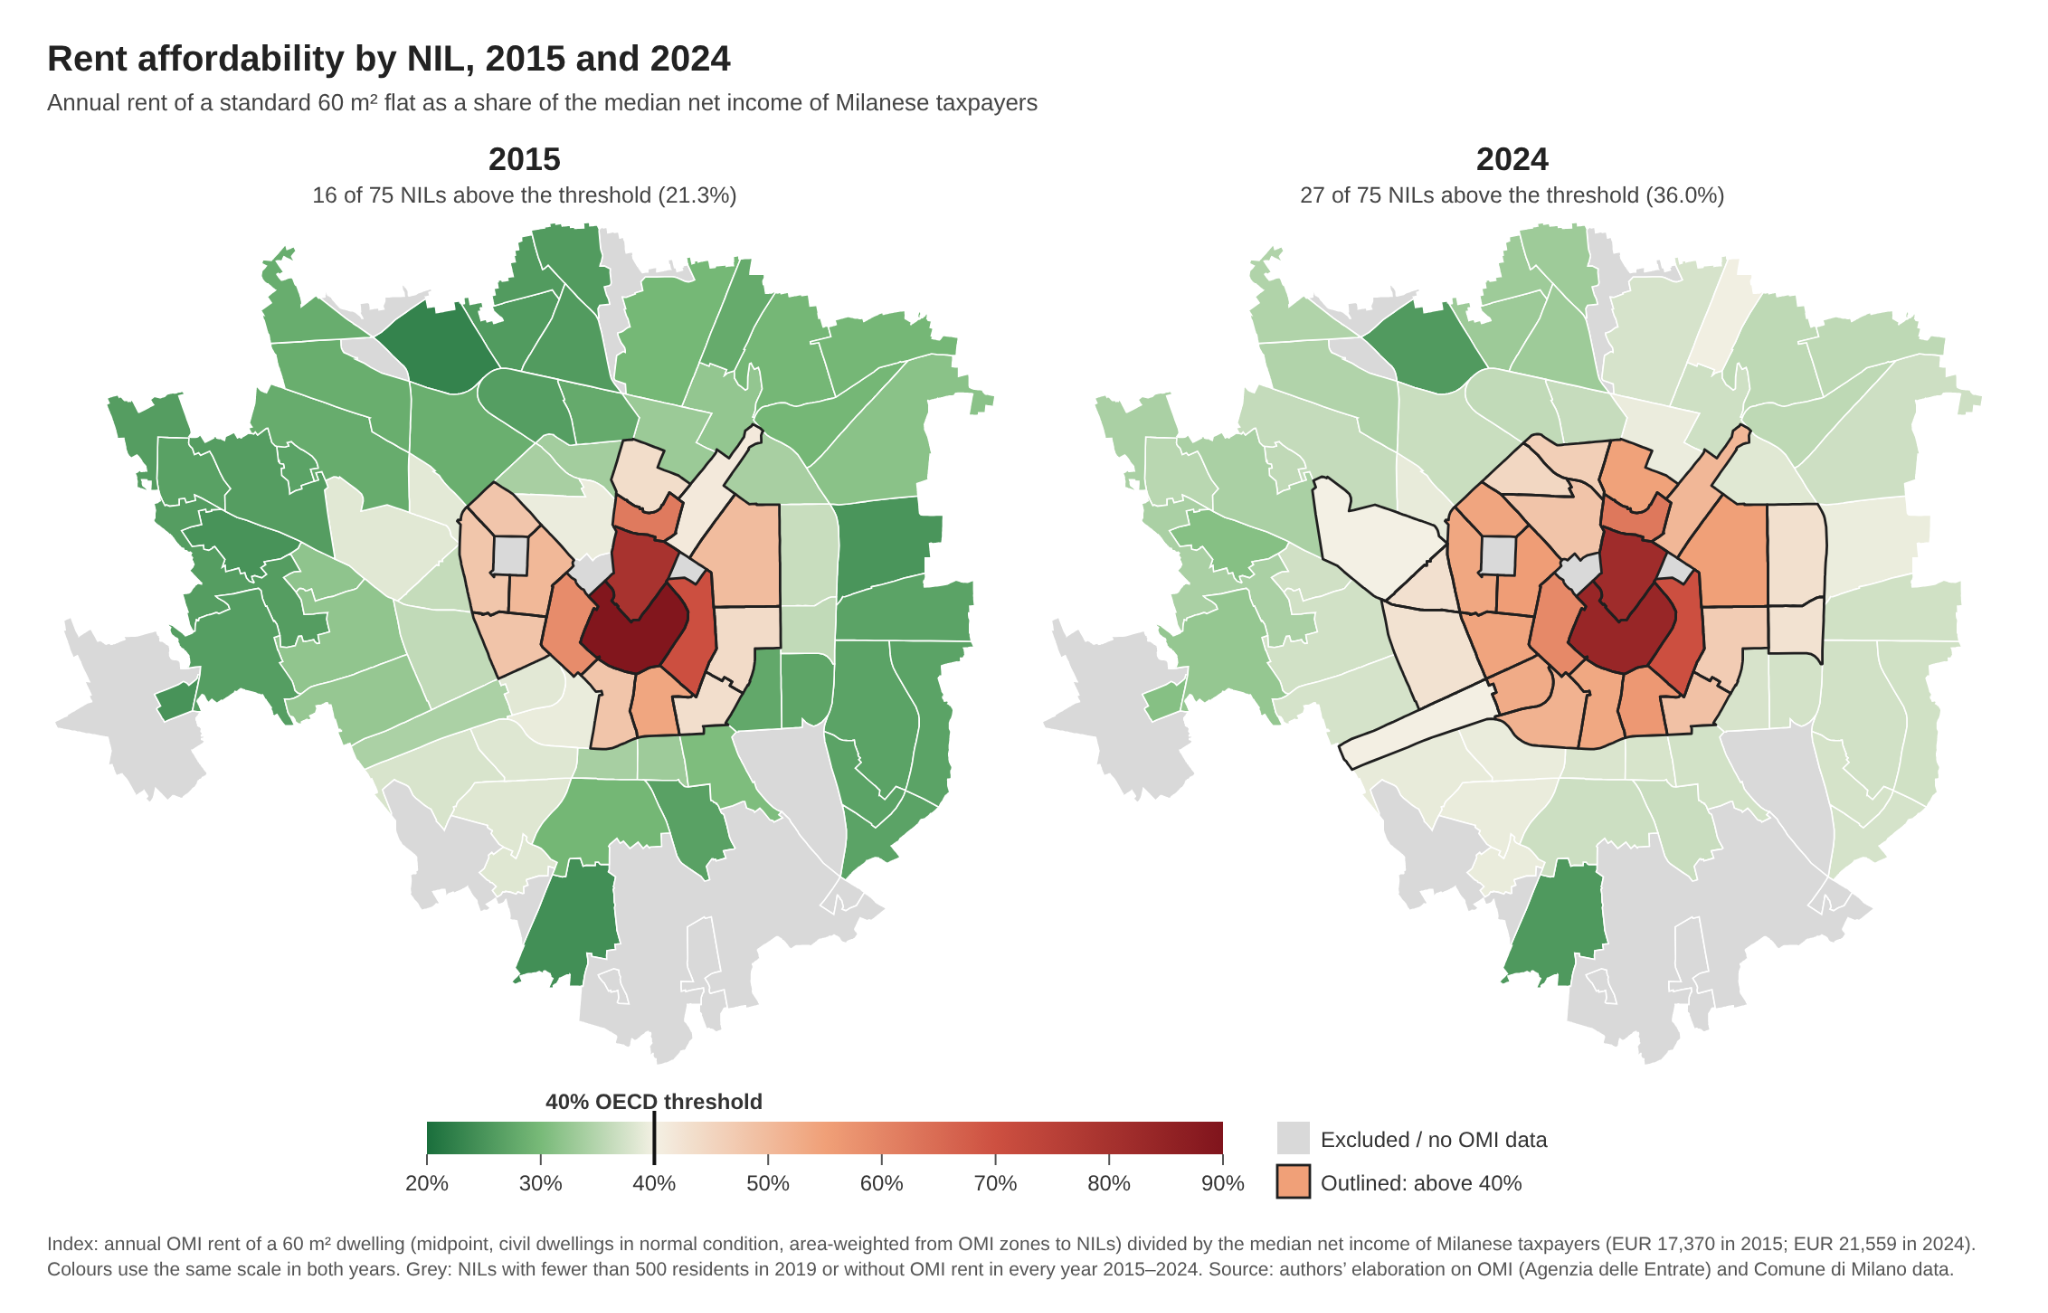
\includegraphics[width=\textwidth]{figures/fig2_map_affordability_2015_2024.png}
\caption{Affordability index by NIL, 2015 and 2024: annual OMI rent of a 60~m$^2$ dwelling (midpoint, civil dwellings in normal condition, area-weighted from OMI zones to NILs) as a share of the median net income of Milanese taxpayers (EUR~17,370 in 2015, EUR~21,559 in 2024). Green: below the 40\% threshold; red: above it; outlined NILs exceed 40\%. The same colour scale is used in both years. Grey: NILs with fewer than 500 residents in 2019 or without an OMI rent in every year 2015--2024. Source: authors' elaboration on OMI and Comune di Milano data.}
\label{fig:map}
\end{figure*}

\begin{table*}[tbhp]
\centering
\caption{NILs in the lower and upper quartiles of the affordability index, 2024}
\label{tab:quartiles}
\resizebox{\textwidth}{!}{%
\begin{tabular}{rlrrrrr}
\toprule
Rank & NIL (code) & Residents & Rent & Annual rent, & Affordability & Affordability \\
 & & 2024 & (EUR/m$^2$/month) & 60 m$^2$ (EUR) & 2024 (\%) & 2015 (\%) \\
\midrule
\multicolumn{7}{l}{\textit{Lower quartile: most affordable ($A\le36.3\%$)}} \\
1 & Gratosoglio -- Q.re Missaglia -- Q.re Terrazze (41) & 18,912 & 7.69 & 5,534 & 25.7 & 24.3 \\
2 & Quarto Oggiaro -- Vialba -- Musocco (76) & 32,744 & 7.73 & 5,569 & 25.8 & 22.8 \\
3 & Muggiano (54) & 3,045 & 9.32 & 6,714 & 31.1 & 24.9 \\
4 & Quinto Romano (62) & 4,744 & 9.33 & 6,714 & 31.1 & 24.9 \\
5 & Baggio -- Q.re degli Olmi -- Q.re Valsesia (55) & 30,860 & 9.68 & 6,971 & 32.3 & 26.3 \\
6 & Bovisasca (81) & 7,584 & 9.87 & 7,110 & 33.0 & 25.9 \\
7 & Comasina (82) & 10,087 & 9.90 & 7,128 & 33.1 & 25.9 \\
8 & Affori (80) & 26,395 & 9.90 & 7,128 & 33.1 & 25.9 \\
9 & Bruzzano (83) & 12,758 & 9.90 & 7,130 & 33.1 & 25.9 \\
10 & Parco Bosco in Citt\`a (88) & 666 & 10.20 & 7,342 & 34.1 & 26.2 \\
11 & Cascina Merlata (73) & 1,130 & 10.35 & 7,450 & 34.6 & 28.3 \\
12 & Maggiore -- Musocco -- Certosa (72) & 9,930 & 10.37 & 7,468 & 34.6 & 28.4 \\
13 & Figino (63) & 2,637 & 10.57 & 7,610 & 35.3 & 26.7 \\
14 & Adriano (17) & 18,169 & 10.68 & 7,687 & 35.7 & 29.6 \\
15 & Padova -- Turro -- Crescenzago (19) & 38,167 & 10.68 & 7,687 & 35.7 & 29.6 \\
16 & Gorla -- Precotto (16) & 30,101 & 10.68 & 7,688 & 35.7 & 29.6 \\
17 & Trenno (64) & 3,986 & 10.73 & 7,722 & 35.8 & 26.9 \\
18 & Bovisa (77) & 13,879 & 10.75 & 7,739 & 35.9 & 26.3 \\
19 & Q.re Gallaratese -- Q.re San Leonardo -- Lampugnano (65) & 33,236 & 10.83 & 7,796 & 36.2 & 28.2 \\
\midrule
\multicolumn{7}{l}{\textit{Upper quartile: least affordable ($A\ge46.5\%$)}} \\
57 & XXII Marzo (26) & 31,477 & 13.97 & 10,059 & 46.7 & 43.9 \\
58 & Sarpi (69) & 30,942 & 14.43 & 10,387 & 48.2 & 39.3 \\
59 & Porta Romana (27) & 16,367 & 14.59 & 10,506 & 48.7 & 43.4 \\
60 & Stazione Centrale -- Ponte Seveso (10) & 17,543 & 15.20 & 10,942 & 50.8 & 41.3 \\
61 & Porta Ticinese -- Conchetta (44) & 16,593 & 15.46 & 11,130 & 51.6 & 39.2 \\
62 & Porta Genova (50) & 15,170 & 15.85 & 11,410 & 52.9 & 38.6 \\
63 & Porta Ticinese -- Conca del Naviglio (6) & 20,348 & 16.03 & 11,544 & 53.5 & 48.0 \\
64 & De Angeli -- Monte Rosa (58) & 21,552 & 16.09 & 11,584 & 53.7 & 47.9 \\
65 & Portello (67) & 8,925 & 16.18 & 11,646 & 54.0 & 48.0 \\
66 & Porta Magenta (51) & 26,819 & 16.22 & 11,681 & 54.2 & 48.2 \\
67 & Isola (11) & 22,458 & 16.37 & 11,788 & 54.7 & 43.6 \\
68 & Buenos Aires -- Porta Venezia -- Porta Monforte (21) & 62,520 & 16.49 & 11,870 & 55.1 & 49.8 \\
69 & Pagano (68) & 17,768 & 16.63 & 11,971 & 55.5 & 50.5 \\
70 & Porta Vigentina -- Porta Lodovica (5) & 13,537 & 16.90 & 12,169 & 56.4 & 53.9 \\
71 & Magenta -- S.~Vittore (7) & 18,026 & 17.76 & 12,789 & 59.3 & 58.7 \\
72 & Porta Garibaldi -- Porta Nuova (9) & 5,817 & 18.73 & 13,488 & 62.6 & 62.1 \\
73 & Guastalla (4) & 15,470 & 21.05 & 15,158 & 70.3 & 70.4 \\
74 & Brera (2) & 18,361 & 24.53 & 17,659 & 81.9 & 79.7 \\
75 & Duomo (1) & 16,226 & 25.11 & 18,082 & 83.9 & 89.4 \\
\bottomrule
\end{tabular}}
\addtabletext{Affordability: annual OMI rent of a 60~m$^2$ dwelling as a share of the median net income of Milanese taxpayers (index $A_{it}$, Eq.~\ref{eq:index}). Rank among the 75 NILs of the balanced sample, from most to least affordable in 2024. Source: authors' elaboration on OMI and Comune di Milano data.}
\end{table*}

\subsection*{What Can a Median Earner Afford?}

The 40\% threshold translates into a monthly rent budget. With one median net income, a household can spend up to EUR~719 per month in 2024 (EUR~579 in 2015); with two median incomes, EUR~1,437. Dividing by the dwelling size gives the highest rent per square metre that remains affordable (Table~\ref{tab:scenarios}). A single median earner looking for a 60~m$^2$ flat can afford rents up to EUR~11.98 per m$^2$ in 2024, which is the case in 48 of the 75 NILs (64\%), down from 59 in 2015. The same person in a 40~m$^2$ flat can pay up to EUR~17.97 per m$^2$ and is priced out of only four central NILs (Duomo, Brera, Guastalla and Porta Garibaldi--Porta Nuova) in both years. A couple with two median incomes renting 60~m$^2$ can pay up to EUR~23.95 per m$^2$ and is excluded only from Duomo and Brera in 2024 (Duomo alone in 2015).

The scenarios therefore change the level of the problem rather than its geography: because the three indices are proportional, they rank NILs identically and differ only in how many lie above the line. The decline in affordability between 2015 and 2024 is concentrated on one-income households seeking a family-size dwelling, for whom more than a third of NILs are now out of reach.

\begin{table}[tbhp]
\centering
\caption{Affordability under alternative household scenarios, 2015 and 2024}
\label{tab:scenarios}
\resizebox{\columnwidth}{!}{%
\begin{tabular}{lccccc}
\toprule
 & Budget & \multicolumn{2}{c}{Max. rent (EUR/m$^2$)} & \multicolumn{2}{c}{Affordable NILs (of 75)} \\
\cmidrule(lr){3-4}\cmidrule(lr){5-6}
Scenario & 2024 (EUR) & 2015 & 2024 & 2015 & 2024 \\
\midrule
One earner, 60 m$^2$ (main) & 719 & 9.65 & 11.98 & 59 & 48 \\
One earner, 40 m$^2$ & 719 & 14.47 & 17.97 & 71 & 71 \\
Two earners, 60 m$^2$ & 1,437 & 19.30 & 23.95 & 74 & 73 \\
\bottomrule
\end{tabular}}
\addtabletext{Budget: monthly rent equal to 40\% of monthly median net income (one or two incomes). Maximum rent: budget divided by dwelling size, per month. Affordable: index $\le$ 40\%. The index uses quoted rents and a citywide individual income, so it describes where a median earner could rent, not the burden of current residents. Source: authors' elaboration on OMI and Comune di Milano data.}
\end{table}

The level of the index also depends on how net income is simulated. Under the alternative tax assumptions in the Appendix (Table~\ref{tab:affdeduct}), the share of residents above the threshold in 2024 ranges from 0.40, with net income calibrated to the taxes actually paid, to 0.81, with no tax credits or with gross income and a 30\% threshold. Two features hold in every scenario: the calibrated scenario almost coincides with the baseline, so the choice of employee tax credits does not drive the results, and every scenario shows a broadly stable share until 2022 followed by a sharp rise in 2023--2024.

\subsection*{Did the M4 Raise Rents in Newly Served Areas?}

Rents did not increase in the newly served zones after the M4 opened. Over the semesters observed after opening, rents in the five newly served OMI zones grew 4.6\% less than in their matched controls (ATT $=-0.047$ log points; permutation $p=0.13$). Inverting the permutation test under a constant effect, effects outside $[-9.7\%,+2.2\%]$ are rejected at the 5\% level: relative rent increases larger than about 2\% are inconsistent with the data, while decreases of up to about 10\% cannot be ruled out. The average pre-opening coefficient over $e=-8,\dots,-2$ is $+0.028$ log points ($p=0.52$).

Fig.~\ref{fig:event} shows the event study. Before opening, rents in the M4 zones were between about 2.5 and 6.5 log points above the matched controls from $e=-12$ to $e=-7$ and converged steadily to zero by $e=-1$. No pre-opening coefficient is individually significant and the simultaneous band contains zero for all of them, but the point estimates trace a gradual relative decline that started years before the line opened, and the pre-test has little power with five treated zones. After opening, the first three coefficients are $-0.035$ (95\% CI $-0.072$ to $+0.002$), $-0.036$ and $-0.054$, all with intervals that include zero. From $e=+3$ to $+6$ the coefficients rest on a single zone (D12, section 1), so the further fall to $-0.09$ reflects the change in composition rather than a growing effect. Taken together, the post-opening estimates are consistent with the continuation of the pre-existing relative decline and cannot be attributed to the line.

\begin{figure*}[tbhp]
\centering
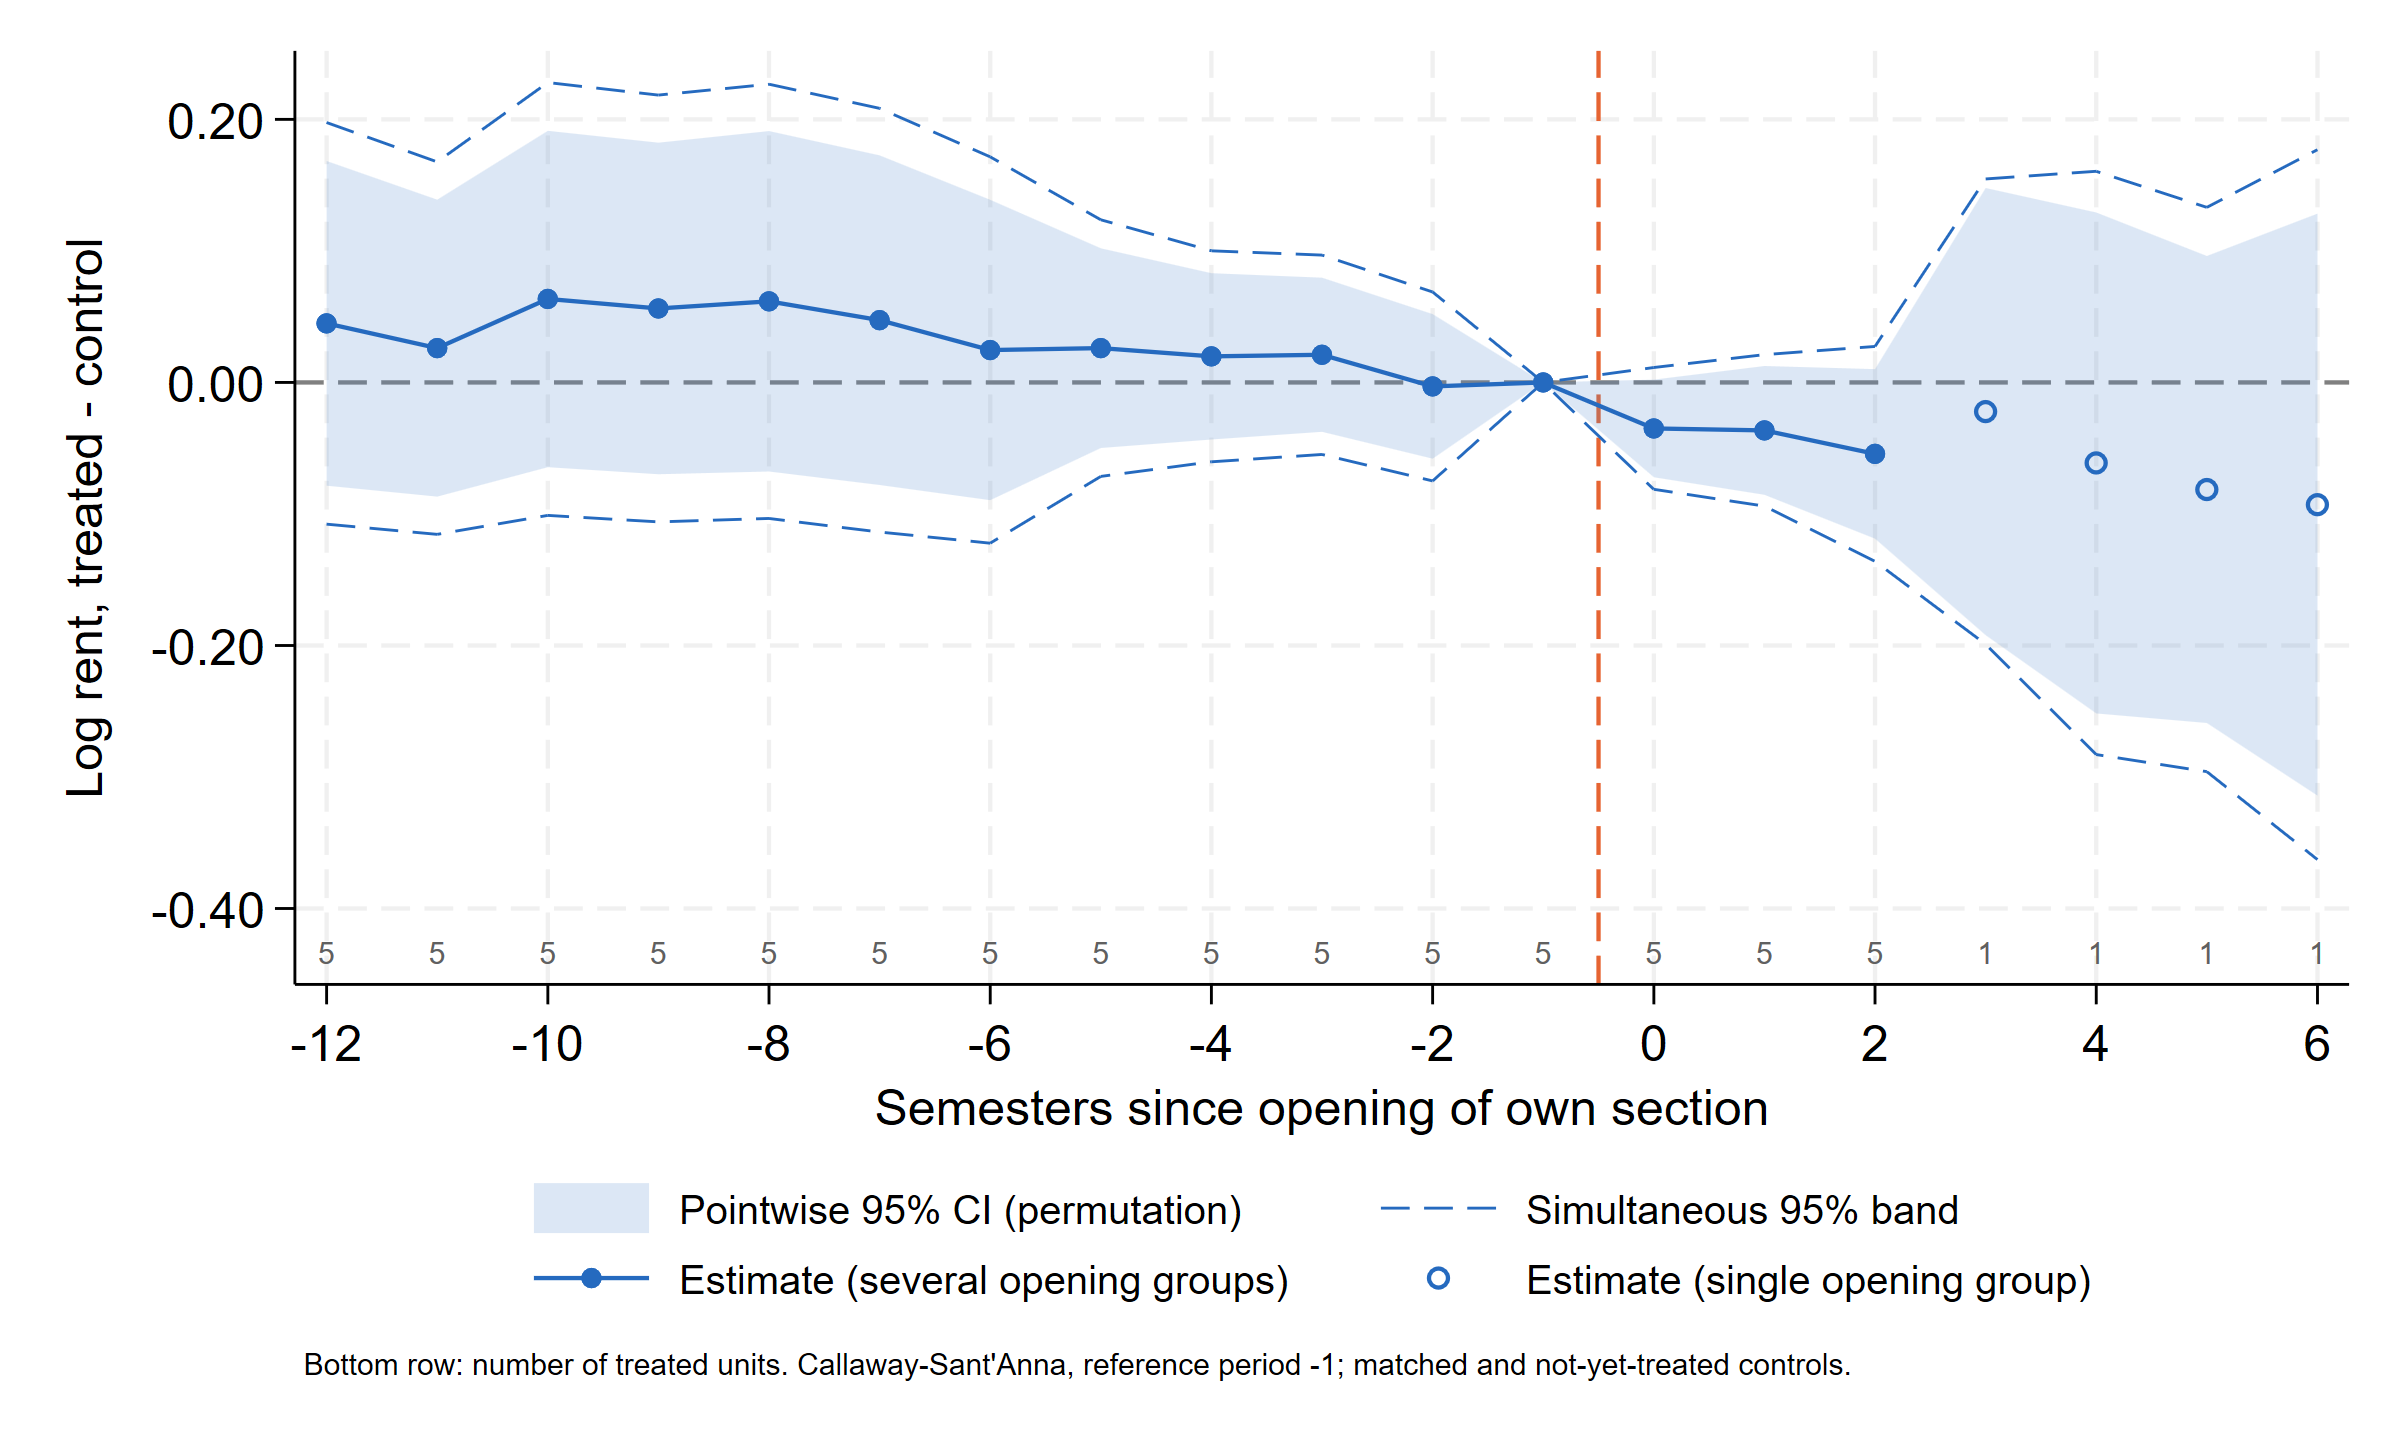
\includegraphics[width=0.8\textwidth]{figures/fig3_m4_event_study_rent.png}
\caption{Event study: log OMI rent in zones newly served by the M4 relative to matched and not-yet-treated controls. Callaway--Sant'Anna coefficients by semester relative to opening (reference $e=-1$). Shaded area: approximate pointwise 95\% intervals; dashed lines: approximate 95\% simultaneous sup-$t$ band over $e=-12,\dots,6$, both from 999 permutations of the opening groups. Bottom row: number of treated zones in each coefficient; hollow markers rest on a single opening group. Sample: 11 OMI zones, 2014S2--2026S1.}
\label{fig:event}
\end{figure*}

The alternative specifications and robustness checks reported in the Appendix (Tables~\ref{tab:m4controls}--\ref{tab:m4sdid}) have four main implications. First, the result does not depend on the matching: with all 20 never-exposed zones as controls the estimate is $-4.0\%$ ($p=0.24$), while using only zones that open later gives an imprecise and uninformative $+3.2\%$ (approximate CI $-4.6\%$ to $+11.7\%$), based on one treated zone over four semesters. Second, it does not depend on the exact treatment definition: with catchments of 800 or 1,000~m and exposure thresholds of 10\% or 30\%, the estimate stays between $-1\%$ and $-6\%$; it becomes significant only with the 10\% threshold, which doubles the number of treated zones ($-4.6\%$, $p=0.036$). Third, it is not driven by a single zone or by the classification of opening periods: leaving out one treated zone at a time gives estimates between $-3.6\%$ and $-5.6\%$, and using $g-2$ as reference or dating treatment from the opening semester gives $-4.4\%$ and $-3.5\%$. Fourth, synthetic difference-in-differences gives $-3.8\%$ (95\% CI $-10.2\%$ to $+3.0\%$), close to the main estimate, after reducing the pre-opening gap between treated and weighted controls from 0.054 to 0.015 log points; the much larger $-12.2\%$ of a two-way fixed-effects regression comes from its reference period rather than from the staggered timing. No check points to a rent increase in the newly served zones.

% ============================================================================
% DISCUSSION
% ============================================================================
\section*{Discussion}

\subsection*{Rental Affordability Across Neighbourhoods}

Measured against the income of the median Milanese taxpayer, renting a standard family-size dwelling became markedly harder after 2022. Until then, the share of residents living in neighbourhoods out of reach was broadly stable at 25--30\%; by 2024 it had reached 43\%. The cause is the gap between quoted rents, which rose by almost a third in two years, and incomes, which grew by less than a tenth. The geography of unaffordability is stable, centred on the historic core and its first ring, but the deterioration also reached peripheral neighbourhoods that remain below the threshold, consistent with evidence that housing costs in Milan have grown faster than incomes \cite{bricocoli2024}. A single earner can still find a 60~m$^2$ dwelling within budget in about two-thirds of the neighbourhoods, almost all of them peripheral; a couple with two median incomes, or a single person in a small flat, is excluded only from the most central areas.

These results describe access to the rental market for a person with the benchmark income, not the situation of current residents. Four features of the index bound their interpretation. The numerator is an appraisal-based quotation for a hypothetical dwelling rather than rents actually paid, and new contracts may differ from quotations. The denominator is a simulated individual income at the median taxpayer rank, which excludes household-specific deductions and transfers; its level depends on the tax assumptions, although the timing and geography of the deterioration do not. Neighbourhood rents are surface-weighted averages of zone quotations, so they are not weighted by dwellings or tenants. Finally, the 40\% threshold follows the OECD overburden convention but is applied to an individual taxpayer income rather than to household disposable income.

\subsection*{The M4 Line}

In the five newly served OMI zones and over the first three to seven semesters after opening, we find no robust evidence of an increase in rent quotations attributable to the M4, relative to comparable zones. Under the maintained assumptions, relative increases larger than about 2\% are inconsistent with the data, but the estimates cannot distinguish a zero effect from a moderate decrease. The negative point estimates should not be read as a causal fall in rents either: the relative decline of the served zones began before the line opened, and the design cannot separate a possible effect of the line from that trend. For the affordability question, the 2022--2024 rise in rents does not appear to be concentrated in the zones newly served by the M4; because the design identifies a relative effect, however, it cannot speak to effects of the line common to the whole city.

Several features of the setting limit these conclusions. First, only five zones are treated, so power reaches 80\% only for effects of about $\pm9\%$, larger than the modest and very local effects found in part of the literature on new rail lines \cite{gibbons2005,billings2011}. Second, the post-opening period is short: seven semesters for section 1 and three for section 3. Third, the permutation $p$-value has exact level only if opening dates are exchangeable across the sample zones, which the route of the line does not guarantee: newly served zones are mostly central while clean controls are more peripheral, so a divergence between centre and periphery over the same years is confounded with the effect of the line, and the positive pre-opening placebo points in this direction. Fourth, the reference semester was already partly served for two sections, although excluding it does not change the estimate. Fifth, the line was announced and construction began before 2014, so any capitalisation at announcement, of the kind documented for other lines \cite{mcmillen2004}, predates our panel and is not captured. Sixth, OMI zones are much larger than a station's walking catchment, which dilutes a local effect; station-level listing data would allow a sharper test.

\subsection*{Conclusion}

Rental affordability in Milan deteriorated sharply after 2022: by 2024 more than four residents in ten lived in neighbourhoods where the rent of a standard 60~m$^2$ dwelling exceeded 40\% of the median taxpayer's net income, up from a quarter in 2015, and even the most affordable peripheral neighbourhoods moved closer to the threshold. The opening of the M4 does not appear to be a driver of this deterioration: in the sample and horizon observed, we find no robust evidence that the line raised rent quotations in the areas it newly served, although the data cannot rule out small effects in either direction. Because the deterioration is citywide rather than concentrated around new infrastructure, the evidence points to affordability policies operating at the city level, while longer post-opening periods and finer spatial data will be needed to assess the local housing effects of the M4.

\subsection*{Data, Materials, and Software Availability}
All data are public: OMI quotations from the Agenzia delle Entrate and Comune di Milano open data (DS1996), taxpayer income classes (DS531), tax totals (DS312), neighbourhood population and composition (DS205, DS27, DS1440, DS1600, DS1956) and metro stations (DS535). The Stata code that reproduces every table and figure is available from the authors. % CHECK: add repository link if the code is made public

% References cited in the verbatim Literature Review (author-year text):
\nocite{bancaditalia2026,hulchanski1995,scottishgov2019,oecd2024,bricocoli2024,bricocoli2025,zheng2013,mcmillen2004,melser2020,callaway2021,padeiro2019,bricocoli2016,bortolotti2025}

\bibsplit[3]
\bibliography{references}

% ============================================================================
% APPENDIX (SUPPORTING INFORMATION)
% ============================================================================
\clearpage
\section*{Appendix: Supporting Information}
\renewcommand{\thetable}{S\arabic{table}}
\setcounter{table}{0}

This appendix reports the alternative specifications, robustness checks and sensitivity analyses summarised in the Results. Unless stated, M4 estimates use the log OMI midpoint rent, the Callaway--Sant'Anna estimator with matched and not-yet-treated controls and permutation inference.

\subsection*{M4: Alternative Control Groups}

Table~\ref{tab:m4controls} compares the main estimate with two specifications that differ only in the control group. Specification (2) uses all 20 never-exposed zones instead of the six matched ones, to test whether the result depends on the matching; the estimate is very similar. Specification (3) uses only zones of sections that open later, which were selected by the same planning process; once the last section opens no control is left, so it compares the single section-1 zone with the four section-3 zones up to 2024S2. Its estimate is positive but very imprecise, and we treat it as uninformative rather than as contradicting (1) and (2). The minimum detectable effect is 9.4\% for (1) and 9.2\% for (2). It is not monotone in the length of the post-period (8.7\% with the sample ending in 2025S2, 9.4\% ending in 2026S1), because quotations move in persistent steps and an additional semester does not mechanically add independent information.

\begin{table*}[tbhp]
\centering
\caption{Effect of the M4 opening on log rents: alternative control groups (Callaway--Sant'Anna)}
\label{tab:m4controls}
\resizebox{\textwidth}{!}{%
\begin{tabular}{llcccccc}
\toprule
 & Controls & ATT & 95\% CI & Permutation & Pre-opening & Treated / never- & Period \\
 & & & & $p$ & placebo ($p$) & exposed controls & \\
\midrule
(1) Main & Matched + not-yet-treated & $-4.6\%$ & $[-9.7\%, +2.2\%]$ & 0.133 & $+0.028$ (0.52) & 5 / 6 & 2014S2--2026S1 \\
(2) & All never-exposed + not-yet-treated & $-4.0\%$ & $[-9.6\%, +2.4\%]$ & 0.243 & $+0.052$ (0.20) & 5 / 20 & 2014S2--2026S1 \\
(3) & Not-yet-treated only & $+3.2\%$ & $[-4.6\%, +11.7\%]^{a}$ & 0.625 & $-0.045$ (0.62) & 5 / 0 & 2014S2--2024S2 \\
\bottomrule
\end{tabular}}
\addtabletext{Outcome: log OMI midpoint rent; OMI zones, semesters. Percentages are $100\times(\exp(\mathrm{ATT})-1)$. Permutation $p$-values from 999 random relabellings of the opening groups. 95\% intervals invert the permutation test under a constant additive effect; $^{a}$approximate interval (estimate $\pm c$). Placebo: average pre-opening coefficient over $e=-8,\dots,-2$, in log points.}
\end{table*}

\subsection*{M4: Two-Way Fixed Effects}

A two-way fixed-effects regression of log rent on a treatment indicator, with zone and semester fixed effects and standard errors clustered by zone, on the five treated and 20 never-exposed zones, gives $-12.2\%$ (cluster-robust 95\% CI $-21.5\%$ to $-1.8\%$). The gap with the main estimate does not come from the staggered timing: a plain difference-in-differences, which makes no comparison between already-treated and later-treated zones, gives a similar value ($-12.5\%$, Table~\ref{tab:m4sdid}). It comes from the reference period, which for these regressions is the average of all pre-opening semesters, during which the served zones were declining relative to the controls, whereas Callaway--Sant'Anna compares each post-opening semester with the semester before opening. With five clusters, the cluster-robust interval is not reliable \cite{conley2011,mackinnon2018}.

\subsection*{M4: Robustness Checks}

Table~\ref{tab:m4robust} reports the checks on the treatment definition, influential zones and the classification of opening periods. The estimate is similar with an 800~m catchment or a 10\% or 30\% exposure threshold, and smaller with a 1,000~m catchment. With the 10\% threshold the number of treated zones doubles to ten and the estimate becomes significant ($-4.6\%$, $p=0.036$), with the same sign and size as the main estimate. Dropping one treated zone at a time keeps the estimate between $-3.6\%$ and $-5.6\%$, with $p$-values between 0.05 and 0.23. The reference semester is partly treated for two sections: 2022S2 was served for 20\% of its days (section 1) and 2024S2 for 44\% (section 3). Using $g-2$ as reference gives $-4.4\%$; dating treatment from the opening semester itself gives $-3.5\%$.

\begin{table}[tbhp]
\centering
\caption{M4 robustness checks, log rent}
\label{tab:m4robust}
\begin{tabular}{lccc}
\toprule
Check & Estimate & $p$ & Treated \\
\midrule
Main specification (1) & $-4.6\%$ & 0.13 & 5 \\
Catchment 800 m & $-5.2\%$ & 0.42 & 3 \\
Catchment 1,000 m & $-1.3\%$ & 0.80 & 4 \\
Exposure threshold 10\% & $-4.6\%$ & 0.036 & 10 \\
Exposure threshold 30\% & $-4.2\%$ & 0.32 & 2 \\
Leave one treated zone out & $-3.6$ to $-5.6\%$ & 0.05--0.23 & 4 \\
Reference period $g-2$ & $-4.4\%$ & 0.40 & 5 \\
Treatment from opening semester & $-3.5\%$ & 0.45 & 5 \\
Synthetic DiD & $-3.8\%$ & 0.27 & 5 \\
\bottomrule
\end{tabular}
\addtabletext{Callaway--Sant'Anna with matched and not-yet-treated controls and permutation $p$-values, unless stated. Catchment and threshold variants use 499 permutations. The synthetic DiD uses all never-exposed zones; its $p$-value comes from placebo standard errors and a normal approximation.}
\end{table}

\subsection*{M4: Synthetic Difference-in-Differences}

On the same balanced sample and horizon (5 treated and 20 never-exposed zones), Table~\ref{tab:m4sdid} compares synthetic difference-in-differences with Callaway--Sant'Anna and a plain difference-in-differences. The pre-trend is the mean of $[(\text{treated}-\text{control})_t-(\text{treated}-\text{control})_{g-1}]$ over $e=-8,\dots,-2$, measured in the same way for all methods. The plain difference-in-differences, which uses the average of all pre-opening semesters as reference, is much more negative. Once controls and periods are reweighted, the pre-trend falls from 0.054 to 0.015 log points and the estimate is close to Callaway--Sant'Anna and not significant. Unit weights spread over about 11 effective controls, with a maximum weight of 0.17; time weights concentrate on the semester before opening (66\% for section 1, 97\% for section 3).

\begin{table}[tbhp]
\centering
\caption{Same sample and horizon: Callaway--Sant'Anna, difference-in-differences and synthetic DiD}
\label{tab:m4sdid}
\resizebox{\columnwidth}{!}{%
\begin{tabular}{lcccc}
\toprule
Method & Estimate & 95\% CI & $p$ & Pre-trend \\
\midrule
C\&S, never-exposed controls & $-4.1\%$ & $[-10.4\%, +2.7\%]$ & 0.23 & $+0.054$ \\
Difference-in-differences & $-12.5\%$ & $[-21.6\%, -2.4\%]$ & 0.017 & $+0.054$ \\
Synthetic DiD & $-3.8\%$ & $[-10.2\%, +3.0\%]$ & 0.27 & $+0.015$ \\
\bottomrule
\end{tabular}}
\addtabletext{5 treated and 20 never-exposed zones, 2014S2--2026S1. C\&S: permutation $p$ and approximate interval (estimate $\pm c$); difference-in-differences and synthetic DiD: placebo standard errors (500 replications) and normal approximation.}
\end{table}

\subsection*{M4: Other Outcomes}

With the same design we also examined OMI sale prices (OMI zones, semesters) and resident out-migration (NILs, years). Out-migration is measured as registered departures to other Italian municipalities per 1,000 residents of the previous year (DS1600, DS1956, DS205), excluding moves abroad and administrative removals. The exposure rule, applied to NILs with annual opening years, assigns three NILs to 2023 and five to 2025; each is matched to the three most similar never-exposed NILs on 2014 composition and 2011 education. Because registry data end in 2024, only the three NILs of the first opening contribute post-opening observations (2023--2024). Neither outcome shows a robust effect. Sale prices grew 3.1\% less in served zones ($p=0.27$). Out-migration fell by 2.4 departures per 1,000 residents ($p=0.07$); the estimate is sensitive to the specification, becoming significant with the 800~m catchment and with the 10\% threshold ($p=0.008$ in both) but falling to $-1.0$ ($p=0.51$) with an earlier reference year. Registered departures do not identify involuntary displacement.

\subsection*{Further Analysis: Net Income under Alternative Tax Assumptions}

Municipal data report only gross total income by class (DS531) and do not say whether a taxpayer is an employee, a pensioner or self-employed, so net income requires an assumption about the tax credits that apply. Survey measures such as the Bank of Italy's household survey avoid this step because respondents report net amounts directly, but they are not representative at the municipal or neighbourhood level. The baseline index applies the employee tax credits. Here we recompute it under four alternatives: (\textit{i}) pension tax credits; (\textit{ii}) self-employment tax credits; (\textit{iii}) no tax credits, which gives the highest possible tax and therefore a lower bound for net income; and (\textit{iv}) a scenario calibrated to the taxes actually paid in Milan, in which the tax at the median is the employee-scenario tax scaled by the ratio of the taxes actually paid by all Milanese taxpayers (DS312) to the taxes the employee model attributes to them. This ratio, between 0.85 and 0.88 in 2015--2024, captures all deductions actually claimed, under the assumption that they weigh proportionally on all incomes. We also report the gross-income version of the index with a 30\% threshold, which requires no tax assumption.

Table~\ref{tab:affdeduct} reports the median income and the share of residents living in NILs where a 60~m$^2$ dwelling costs more than the threshold. The level of the index depends on the tax assumption: in 2024 the share ranges from 0.40 with the calibrated scenario to 0.81 without tax credits or with gross income. Two results hold in every scenario. First, the scenario calibrated to actual taxes gives almost the same shares as the baseline. Second, all scenarios show a broadly stable share between 2015 and 2022 followed by a sharp rise in 2023--2024; scenarios with lower net income show a larger rise, because more neighbourhoods lie close to the threshold.

\begin{table}[tbhp]
\centering
\caption{Affordability under alternative tax assumptions}
\label{tab:affdeduct}
\resizebox{\columnwidth}{!}{%
\begin{tabular}{lcccc}
\toprule
 & Median income & \multicolumn{3}{c}{Share of residents above threshold} \\
\cmidrule(lr){3-5}
Scenario & 2024 (EUR) & 2015 & 2022 & 2024 \\
\midrule
Employee tax credits (baseline) & 21,559 & 0.25 & 0.30 & 0.43 \\
Calibrated to actual taxes & 22,152 & 0.25 & 0.30 & 0.40 \\
Pension tax credits & 20,278 & 0.31 & 0.31 & 0.59 \\
Self-employment tax credits & 19,965 & 0.34 & 0.35 & 0.67 \\
No tax credits & 19,394 & 0.39 & 0.36 & 0.81 \\
Gross income, 30\% threshold & 25,919 & 0.34 & 0.36 & 0.81 \\
\bottomrule
\end{tabular}}
\addtabletext{Share of residents living in NILs where the annual OMI rent of a 60~m$^2$ dwelling exceeds 40\% of the median net income of Milanese taxpayers (30\% of gross income in the last row); balanced panel of 75 NILs. Net income: total income minus personal income tax and regional and municipal surcharges, plus the in-work bonus; household-specific deductions are not modelled, except implicitly in the calibrated scenario. Sources: DS531, DS312, OMI.}
\end{table}

\end{document}
